\noindent
\begin{tabular}{cc}
\begin{minipage}[b]{0.60\textwidth}
\begin{exerciseS}[Tubo di Pitot statico]
Dato il condotto a sezione circolare rappresentato in figura, 
determinare la portata in massa d'olio, $\overline{\rho} = 850\ kg/m^3$,
attraverso il condotto stesso sapendo che il diametro del condotto 
\`{e} $d=0.5\ m$, che la differenza di altezza fra i peli liberi 
\`{e} $H=40\ cm$, che il diametro del tubo ``a U'' \`{e} di $2$ mm. 
Si trascuri qualunque effetto dissipativo, si assuma
uniforme la velocit\`{a} in una sezione sufficientemente lontana a monte
e si consideri che nel tubo ``a U'' sia presente aria in condizioni normali.

($\overline{Q}= 467.2\  kg/s$)
\end{exerciseS}
\end{minipage}
&
\begin{minipage}{0.35\textwidth}
   \begin{center}
   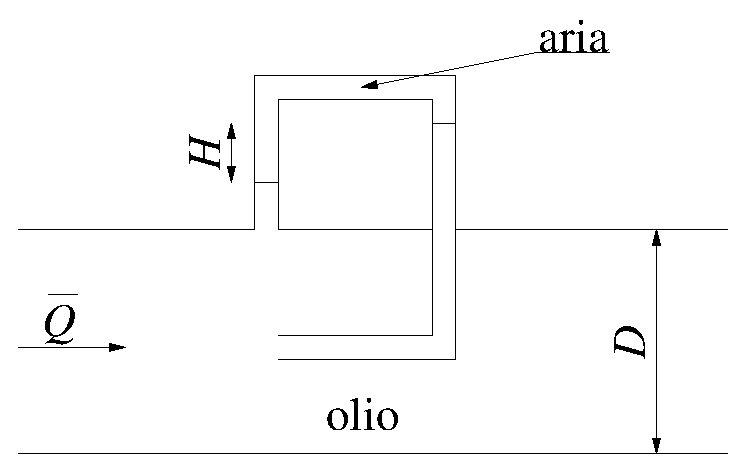
\includegraphics[width=0.90\textwidth]{./fig/condottocircolare.eps}
   \end{center}
\end{minipage}
\end{tabular}

\sol

\partone
 Teorema di Bernoulli nell'ipotesi di stazionarietà, fluido incomprimibile, non viscoso, irrotazionale.
Equazione della vorticità nel caso non viscoso.
Legge di Stevino.

\parttwo
Vengono fatte alcune ipotesi semplificative ($\rho = \bar{\rho}$, $\mu=0$, $\frac{\partial}{\partial t}=0$); si utilizza poi l'equazione della vorticità per semplificare ulteriormente il problema: se si assume che il profilo di velocità all'ingresso sia uniforme, e quindi a vorticità nulla, il fluido nel canale rimane irrotazionale (dall'equazione della vorticità per fluidi non viscosi).

Gli unici due punti che possono creare problemi sono i collegamenti del tubo con il canale.
Sulla linea di corrente che incontra l'imbocco del tubicino, il fluido subisce un rallentamento dalla velocità di ingresso fino ad arrestarsi: su questa linea di corrente è possibile applicare il teorema di Bernoulli.
In corrispondenza del'altro collegamento, si incontra una superficie di discontinuità a vorticità infinita: non è quindi possibile attraversare questa superficie applicando direttamente il teorema di Bernoulli, ma bisogna ricorrere alle condizioni di interfaccia tra i due domini, quello interno al canale e quello interno al tubo, nel quale possono essere applicate le equazioni della statica.

Vengono definiti i punti  $A$  all'ingresso sulla linea di corrente che arriva alla presa del tubo all'interno del canale; il punto $B$ coincidente con la presa del tubo all'interno del canale; $C$ il pelo libero di destra all'interno del tubo ``a U'', $D$ il pelo libero di sinistra. Si definiscono anche $h_C$ e $h_D$ come quote dei peli liberi (oss. $H = h_C - h_D$).

\begin{center}
  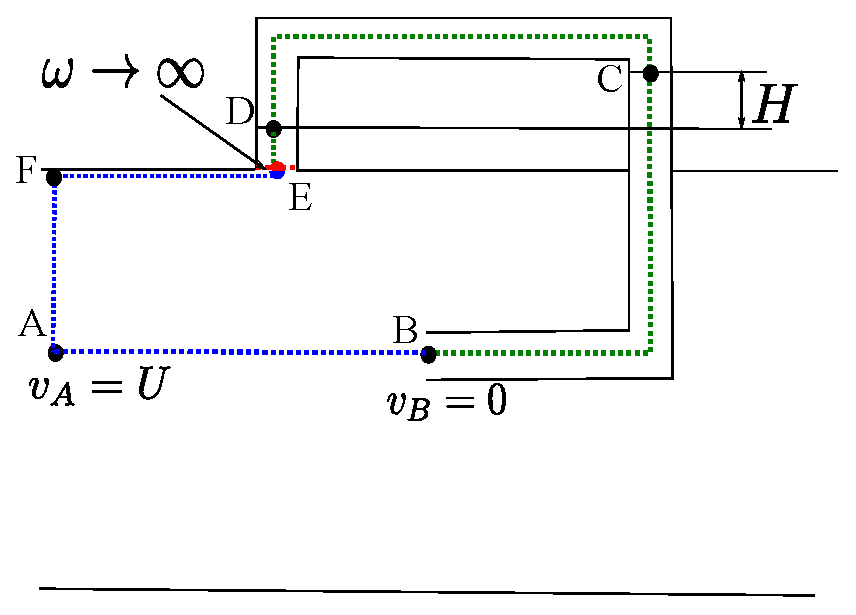
\includegraphics[width=0.35\textwidth]{./fig/Canale01.eps}
\end{center}

Il sistema risolvente è:
\begin{equation}
\begin{cases}
  P_A + \frac{1}{2} \rho v_A^2 + \rho g h_A =
   P_B + \frac{1}{2} \rho v_B^2 + \rho g h_B\\
  P_B + \rho g h_B = P_C + \rho g h_C   \\
  P_C + \rho_a g h_C = P_D + \rho_a g h_D\\
  P_D + \rho g h_D = P_{E_2} + \rho g h_{E_2} \\
  P_{E_2} = P_{E_1} \\
  P_{E_1} + \frac{1}{2} \rho u_{E_1}^2 + \rho g h_{E_1} = P_F + \frac{1}{2} \rho u_F^2 + \rho g h_F\\
 P_F + \frac{1}{2} \rho v_F^2 + \rho g h_F = P_A + \frac{1}{2} \rho v_A^2 + \rho g h_A \\
  \bar{Q} = \rho \frac{\pi}{4}d^2 U
\end{cases}
\end{equation}

Osservando che $h_A = h_B$, $h_E = h_F$, $v_A = v_F = U$, 
$v_B = 0$, supponendo $u_E = U$ (ipotizzando dimensioni e intrusività trascurabile della sonda), il sistema semplificato diventa:
\begin{equation}
\begin{cases}
  P_A + \frac{1}{2} \rho U^2  = P_B \\
  P_B + \rho g h_A = P_C + \rho g h_C   \\
  P_C + \rho_a g h_C = P_D + \rho_a g h_D\\
  P_D + \rho g h_D = P_E + \rho g h_E \\
  P_E + \frac{1}{2} \rho u_E^2 = P_F + \frac{1}{2} \rho U^2 \\
 P_F + \rho g h_E = P_A + \rho g h_A \\
  \bar{Q} = \rho \frac{\pi}{4}d^2 U
\end{cases}
\end{equation}

Risolvendo per U, avendo definito $H = h_C - h_D$:
\begin{equation}
  \frac{1}{2} \rho U^2 = P_B - P_A = ... = (\rho - \rho_a) g H \quad \Rightarrow \quad 
  U = \sqrt{2\displaystyle\left(1-\frac{\rho_a}{\rho}\right) g H}
\end{equation}

Inserendo i valori numerici: $U = 2.799 m/s$, $\bar{Q} = 467.15 kg/s$.


